\paragraph{Question 1}
La complexité est de $O(m(n+m))=O(n^4)$ car~:
\begin{itemize}
\item La taille de la coupe augmente d'un sommet à chaque tour, donc
il nous faut $m$ étapes pour trouver la coupe maximum.
\item À chaque tour, on rajoute un également toutes les arêtes
incidentes au sommet rajouté.
\end{itemize}

\paragraph{Question 2}
Montrons que le taux d'approximation est de 2~:
\begin{proof}Soit $(Y_1,Y_2)$ la coupe approximative. Supposons pour $\Gamma(x)$ l'ensemble des sommets voisins d'un sommet x~:

$\exists x \in Y_1 \text{ | } \Gamma(x) \cap Y_1 > \Gamma(x) \cap Y_2$

Dans un tel cas le déplacement du sommet x dans $Y_2$ augmenterai la valeur de la coupe, donc l'algorithme approché ne l'aurait jamais gardé dans $Y_1$. Notre supposition est donc absurde. Nous avons au contraire~:

$\forall x \in Y_1 \text{ | } \Gamma(x) \cap Y_1 \leq \Gamma(x) \cap Y_2$

Le même raisonnement tient pour les sommets de $Y_2$. Or la somme des degrés est égale à $2|E|$ donc~:

\begin{eqnarray*}
2|E| &=& \Sigma_{x \in Y_1}|\Gamma(x)|  + \Sigma_{x' \in Y_2}|\Gamma(x')| \\
	 &=& \Sigma_{x \in Y_1}[|(\Gamma(x)\cap{} Y_1)|\cup|(\Gamma(x)\cap{}Y_2)|] +
	 	 \Sigma_{x' \in Y_2}[|(\Gamma(x')\cap{} Y_1)|\cup|(\Gamma(x')\cap{}Y_2)|] \\
	 &=& \Sigma_{(x,x') \in (Y_1,Y_2)} +
	 	 \Sigma_{(y,y') \in (Y_2,Y_1)} + 
	 	 \Sigma_{(z,z') \in (Y_1,Y_1)} +
	 	 \Sigma_{(t,t') \in (Y_2,Y_2)} 
\end{eqnarray*}

Or $\Sigma_{(x,x') \in (Y_1,Y_2)} \geq \Sigma_{(z,z') \in (Y_1,Y_1)}$ et $\Sigma_{(y,y') \in (Y_2,Y_1)} \geq \Sigma_{(t,t') \in (Y_2,Y_2)}$ nous avons~:

\begin{eqnarray*}
\Sigma_{(x,x') \in (Y_1,Y_2)} + \Sigma_{(y,y') \in (Y_2,Y_1)} &\geq& |E| \\
\Rightarrow |(Y_1, Y_2)| &\geq& \frac{|E|}{2}
\end{eqnarray*}

Globalement au moins la moitié des arêtes doit donc traverser la coupe
approximative. De plus la coupe optimale est évidement bornée par
$|E|$, donc \mbox{$\frac{(Y_1,Y_2)}{(Y_1,Y_2)^*} \geq \frac{|E|}{2|E|}$},
soit \mbox{$\frac{(Y_1,Y_2)^*}{(Y_1,Y_2)} \geq 2$}, \emph{quod erat
demonstratum}.
\end{proof}

\paragraph{Question 3}

Prenons le graphe figure \ref{coupe_max_instance}. La coupe optimale
(figure \ref{coupe_max_opt}) traverse chacune des 15 arêtes, il suffit
donc de montrer que la coupe approximative n'en traverse que 7.

\begin{figure}[ht]
% LEFT-HAND SIDE
\begin{minipage}[b]{0.5\linewidth}
\centering
\centering
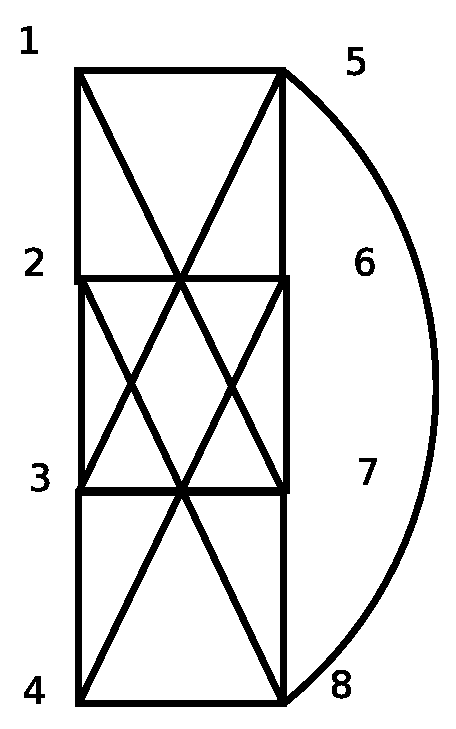
\includegraphics[width=0.4\textwidth]{../images/exo4.eps}
\caption{Instance coupe maximum.}
\label{coupe_max_instance}
\end{minipage}
% RIGHT-HAND SIDE
\hspace{0.5cm}
\begin{minipage}[b]{0.4\linewidth}
\centering
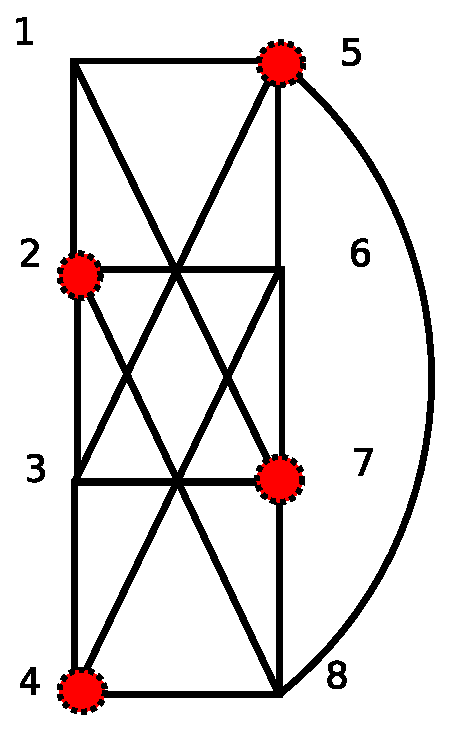
\includegraphics[width=0.5\textwidth]{../images/exo4_opt.eps}
\caption{Coupe optimale.}
\label{coupe_max_opt}
\end{minipage}
\end{figure}

Pour l'instant nous n'avons pas réussi à expliciter une coupe~:

\begin{itemize}
\item de valeur 7,
\item trouvable par l'algorithme approché,
\item sur lequel l'algorithme se bloquerait par la suite.
\end{itemize}

Pourtant l'algorithme n'est pas optimal~: il est bien bloqué sur
$P_4$\footnote{$P_4$ : chemin à quatre sommets} avec une coupe de valeur 2 s'il a la malchance de prendre les deux extrémités (pour $P_4$ la coupe maximum est de 3). Dans ce cas, ce n'est alors un taux
de approximation de $\frac{3}{2}$, mais nous atteignons pas la borne de 2. 

Avec $C_4$\footnote{$C_4$ : cycle à quatre sommets} nous nous bloquerions sur 2 (et pas le maximum 4), donc nous atteindrions la borne, en prenant deux sommets consécutifs\dots sauf que l'algorithme approché ne prendra jamais deux sommets consécutif car ceci n'augmenterait pas la valeur de la coupe.